\documentclass[border=2mm]{standalone}
\usepackage{pgfplots}
\pgfplotsset{compat=1.18}
\definecolor{red}{rgb}{0.7, 0.11, 0.11}
\definecolor{blue}{rgb}{0.0, 0.20, 0.42}
\begin{document}
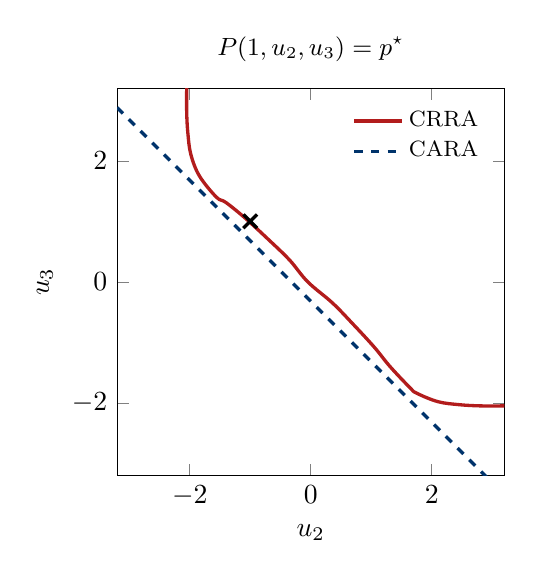
\begin{tikzpicture}
\begin{axis}[
  legend style={draw=none,legend pos=north east,font=\footnotesize},
  xmin=-3.2, xmax=3.2, ymin=-3.2, ymax=3.2,
  xlabel={$u_2$}, ylabel={$u_3$},
  width=6.5cm, height=6.5cm,
  axis equal image,
  title style={font=\small},
  title={$P(1,u_2,u_3)=p^{\star}$}]

% CRRA REE contour (G=14, curved) — use tension spline
\addplot[very thick,color=red,smooth,tension=0.6] coordinates {
  (-2.05,3.20) (-2.05,2.80) (-2.03,2.45) (-1.98,2.10)
  (-1.84,1.75) (-1.56,1.40) (-1.40,1.31) (-1.08,1.05)
  (-0.70,0.70) (-0.35,0.36) (-0.05,0.00)
  (0.36,-0.35) (0.70,-0.70) (1.05,-1.08) (1.31,-1.40)
  (1.64,-1.75) (1.75,-1.84) (2.10,-1.98) (2.45,-2.03)
  (2.80,-2.05) (3.20,-2.05)};

% CARA contour (straight: u2+u3 = const ≈ -0.325)
\addplot[very thick,color=blue,dashed]
  coordinates {(-3.2,2.88) (3.2,-3.52)};

% Actual realization
\addplot[only marks,mark=x,mark size=3.5pt,very thick,color=black]
  coordinates {(-1,1)};

\legend{CRRA, CARA}
\end{axis}
\end{tikzpicture}
\end{document}
